%----------
%   WARNING
%----------

% This Guide contains Library recommendations based mainly on APA and IEEE styles, but you must always follow the guidelines of your TFG Tutor and the TFG regulations for your degree.

% THIS TEMPLATE IS BASED ON THE IEEE STYLE 


%----------
% DOCUMENT SETTINGS
%----------

\documentclass[12pt]{report} % font: 12pt

% Custom packages
\usepackage{comment}
\usepackage[numbers]{natbib}

\bibliographystyle{IEEEtran}


% margins: 2.5 cm top and bottom; 3 cm left and right
\usepackage[
a4paper,
vmargin=2.5cm,
hmargin=3cm
]{geometry}

% Paragraph Spacing and Line Spacing: Narrow (6 pt / 1.15 spacing) or Moderate (6 pt / 1.5 spacing)
\renewcommand{\baselinestretch}{1.15}
\parskip=6pt

% Color settings for cover and code listings 
\usepackage[table]{xcolor}
\definecolor{azulUC3M}{RGB}{0,0,102}
\definecolor{gray97}{gray}{.97}
\definecolor{gray75}{gray}{.75}
\definecolor{gray45}{gray}{.45}

% PDF/A -- Important for its inclusion in e-Archive. PDF/A is the optimal format for preservation and for the generation of metadata: http://uc3m.libguides.com/ld.php?content_id=31389625. 

% In the template we include the file OUTPUT.XMPDATA. You can download that file and include the metadata that will be incorporated into the PDF file when you compile the memoria.tex file. Then upload it back to your project.  
\usepackage[a-1b]{pdfx}

% LINKS
\usepackage{hyperref}
\hypersetup{colorlinks=true,
	linkcolor=black, % links to parts of the document (e.g. index) in black
	urlcolor=blue} % links to resources outside the document in blue

% MATH EXPRESSIONS
\usepackage{amsmath,amssymb,amsfonts,amsthm}

% Character encoding
\usepackage{txfonts} 
\usepackage[T1]{fontenc}
\usepackage[utf8]{inputenc}

% English settings
\usepackage[english]{babel} 
\usepackage[babel, english=american]{csquotes}
\AtBeginEnvironment{quote}{\small}

% Footer settings
\usepackage{fancyhdr}
\pagestyle{fancy}
\fancyhf{}
\renewcommand{\headrulewidth}{0pt}
\rfoot{\thepage}
\fancypagestyle{plain}{\pagestyle{fancy}}

% DESIGN OF THE TITLES of the parts of the work (chapters and epigraphs or sub-chapters)
\usepackage{titlesec}
\usepackage{titletoc}
\titleformat{\chapter}[block]
{\large\bfseries\filcenter}
{\thechapter.}
{5pt}
{\MakeUppercase}
{}
\titlespacing{\chapter}{0pt}{0pt}{*3}
\titlecontents{chapter}
[0pt]                                               
{}
{\contentsmargin{0pt}\thecontentslabel.\enspace\uppercase}
{\contentsmargin{0pt}\uppercase}                        
{\titlerule*[.7pc]{.}\contentspage}                 

\titleformat{\section}
{\bfseries}
{\thesection.}
{5pt}
{}
\titlecontents{section}
[5pt]                                               
{}
{\contentsmargin{0pt}\thecontentslabel.\enspace}
{\contentsmargin{0pt}}
{\titlerule*[.7pc]{.}\contentspage}

\titleformat{\subsection}
{\normalsize\bfseries}
{\thesubsection.}
{5pt}
{}
\titlecontents{subsection}
[10pt]                                               
{}
{\contentsmargin{0pt}                          
	\thecontentslabel.\enspace}
{\contentsmargin{0pt}}                        
{\titlerule*[.7pc]{.}\contentspage}  


% Tables and figures settings
\usepackage{multirow} % combine cells 
\usepackage{caption} % customize the title of tables and figures
\usepackage{floatrow} % we use this package and its \ ttabbox and \ ffigbox macros to align the table and figure names according to the defined style.
\usepackage{array} % with this package we can define in the following line a new type of column for tables: custom width and centered content
\newcolumntype{P}[1]{>{\centering\arraybackslash}p{#1}}
\DeclareCaptionFormat{upper}{#1#2\uppercase{#3}\par}
\usepackage{graphicx}
\graphicspath{{imagenes/}} % Images folder

% Table layout for engineering
\captionsetup*[table]{
	format=upper,
	name=TABLE,
	justification=centering,
	labelsep=period,
	width=.75\linewidth,
	labelfont=small,
	font=small
}

% Figures layout for engineering
\captionsetup[figure]{
	format=hang,
	name=Fig.,
	singlelinecheck=off,
	labelsep=period,
	labelfont=small,
	font=small		
}

% FOOTNOTES
\usepackage{chngcntr} % continuous numbering of footnotes
\counterwithout{footnote}{chapter}

% CODE LISTINGS 
% support and styling for listings. More information in  https://es.wikibooks.org/wiki/Manual_de_LaTeX/Listados_de_código/Listados_con_listings
\usepackage{listings}

% Custom listing
\lstdefinestyle{estilo}{ frame=Ltb,
	framerule=0pt,
	aboveskip=0.5cm,
	framextopmargin=3pt,
	framexbottommargin=3pt,
	framexleftmargin=0.4cm,
	framesep=0pt,
	rulesep=.4pt,
	backgroundcolor=\color{gray97},
	rulesepcolor=\color{black},
	%
	basicstyle=\ttfamily\footnotesize,
	keywordstyle=\bfseries,
	stringstyle=\ttfamily,
	showstringspaces = false,
	commentstyle=\color{gray45},     
	%
	numbers=left,
	numbersep=15pt,
	numberstyle=\tiny,
	numberfirstline = false,
	breaklines=true,
	xleftmargin=\parindent
}

\captionsetup*[lstlisting]{font=small, labelsep=period}
 
\lstset{style=estilo}
\renewcommand{\lstlistingname}{\uppercase{Código}}


% REFERENCES 

% IEEE bibliography setup
\begin{comment}
\usepackage[backend=biber, style=ieee, isbn=false,sortcites, maxbibnames=6, minbibnames=1]{biblatex} % Setting for IEEE citation style, recommended for engineering. "maxbibnames" indicates that from 6 authors truncate the list in the first one (minbibnames) and add "et al." as used in the IEEE style.

\addbibresource{Sections/Bibliography/References.bib} % The references.bib file in which the bibliography used should be
\end{comment}

%-------------
%	DOCUMENT
%-------------

\begin{document}
\pagenumbering{roman} % Roman numerals are used in the numbering of the pages preceding the body of the work.
	
%----------
%	COVER
%----------	
\begin{titlepage}
	\begin{sffamily}
	\color{azulUC3M}
	\begin{center}
		\begin{comment}
		\begin{figure}[H] % UC3M Logo
			\makebox[\textwidth][c]{\includegraphics[width=16cm]{logo_UC3M.png}}
		\end{figure}
		\end{comment}
		\vspace{2.5cm}
		\begin{Large}
			Master Degree in...\\			
			 2020-2021\\ % Academic year
			\vspace{2cm}		
			\textsl{Master Thesis}
			\bigskip
			
		\end{Large}
		 	{\Huge ``Thesis title''}\\
		 	\vspace*{0.5cm}
	 		\rule{10.5cm}{0.1mm}\\
			\vspace*{0.9cm}
			{\LARGE Author's complete name}\\ 
			\vspace*{1cm}
		\begin{Large}
			1st Tutor complete name\\
			2nd Tutor complete name\\
			Place and date\\
		\end{Large}
	\end{center}
	\vfill
	\color{black}
	\fbox{
	\begin{minipage}{\linewidth}
    	\textbf{AVOID PLAGIARISM}\\
    	\footnotesize{The University uses the \textbf{Turnitin Feedback Studio} for the delivery of student work. This program compares the originality of the work delivered by each student with millions of electronic resources and detects those parts of the text that are copied and pasted. Plagiarizing in a TFM is considered a  \textbf{\underline{Serious Misconduct}}, and may result in permanent expulsion from the University.}\end{minipage}}

	% IF OUR WORK IS TO BE PUBLISHED UNDER A CREATIVE COMMONS LICENSE, INCLUDE THESE LINES. IS THE RECOMMENDED OPTION.
\begin{comment}
	\noindent\includegraphics[width=4.2cm]{creativecommons.png}\\ % Creative Commons Logo
\end{comment}
    \footnotesize{This work is licensed under Creative Commons \textbf{Attribution – Non Commercial – Non Derivatives}}
	
	\end{sffamily}
\end{titlepage}

\newpage % blank page
\thispagestyle{empty}
\mbox{}

\newpage % blank page
\thispagestyle{empty}
\mbox{}

%----------
%	ABSTRACT AND KEYWORDS 
%----------	
\renewcommand\abstractname{\large\bfseries\filcenter\uppercase{Summary}}
\begin{abstract}
\thispagestyle{plain}
\setcounter{page}{3}
	
	% Write your abstract
	
	\textbf{Keywords:} % add the keywords
	
	\vfill
\end{abstract}
	\newpage % Blank page
	\thispagestyle{empty}
	\mbox{}


%----------
%	Dedication
%----------	
\chapter*{Dedication}

\setcounter{page}{5}
	
	% Write here	
		
	\vfill
	
	\newpage % blank page
	\thispagestyle{empty}
	\mbox{}
	

%----------
%	TOC
%----------	

%--
% TOC
%-
\tableofcontents
\thispagestyle{fancy}

\newpage % blank page
\thispagestyle{empty}
\mbox{}

%--
% List of figures. If they are not included, comment the following lines
%-
\listoffigures
\thispagestyle{fancy}

\newpage % blank page
\thispagestyle{empty}
\mbox{}

%--
% List of tables. If they are not included, comment the following lines
%-
\listoftables
\thispagestyle{fancy}

\newpage % blankpage
\thispagestyle{empty}
\mbox{}


%----------
%	THESIS
%----------	
\clearpage
\pagenumbering{arabic} % numbering with Arabic numerals for the rest of the document.	

\chapter{Introduction}
\section{Report Structure}

The report is organized in the following structure; first relevant background information regarding measuring the health of a bridge, WSNs, LoRa and LoRawan, and the internet of things will be presented. Following this, the aims and objectives of this report will be outlined. Next, a review of the relevant published literature will be evaluated. The design specifications and methodology for developing protoype one and two will be provided. Results from testing both prototype implementations will be presented and a discussion regarding these results and performance will be provided. Device limitations will be analysed, suggestions for further improvements will be discussed followed by a conclusion. Proceeding the conclusion will be the references and appendices. 
\section{Project Background}

\subsection{Wireless Sensor Networks}
Wireless Sensor Networks (WSNs) are simple, low-cost networks that primarily consist of nodes and a base station \cite{WSN-WaterQual}. WSN nodes usually comprise of some sensing or measuring capability acting as the physical layer, and relay this information via uplink to a base station for processing and then to a network server acting as the network layer. From here, the API from a network cloud service can be used to create GUI's and other applications for researchers and consumers which acts as the application layer. 

Innovating many field of industry and research, these distributed networks of nodes have been valuable in many contexts. For example, the use of ZigBee communication technology for air pollution monitoring \cite{ZigBeeAirPolution} and the use of Bluetooth for communication between end-devices measuring temperature, luminance, carbon dioxide and humidity for energy-saving establishments \cite{BTenergySaving}. Although these WSNs have worked in the past, the future of this technology lies in developing systems that have high scalability and range, something that ZigBee and Bluetooth inherently lack. Cellular and satellite technology are alternate approaches that offer extremely high data rates and range, however these technologies are not practical to implement in most situations due to exceedingly high costs. 

\subsection{Structural Health Monitoring}
Structural Health Monitoring (SHM) is a vital practice for ensuring the safety and longevity of civil and industrial structures \cite{SHM-IoT-Magazine}. SHM involves continuously tracking change in structures which can be attributed to material aging, environmental influences or unforeseen incidents such as traffic accidents or natural disasters. These changes can be tracked using WSNs equipped with appropriate sensor modules, and integrating data transmission capabilities. A survey investigating the implementation of IoT technology for structural health monitoring (SHM) determined that WSN technology has revolutionized the health monitoring in various fields including civil engineering \cite{SHM-IoT-Survey}. WSN  systems can be deployed to measures a vast array of SHM indicators including temperature, velocity, acceleration, frequency and displacement. WSN can be deployed on a structure such as a bridge operating as Internet of Things (IoT) nodes. This deployment highlights the advantage of using WSNs for SHM since the collected data can be uploaded to the cloud for processing and distribution. Within the context of bridge monitoring, the integration of WSN with IoT for SHM can serve various application requirements for real-time data uplink such as monitoring acceleration and frequency characteristics. This data can be plotted on a continuous time spectrum and compared to observational data such as pedestrian load to verify the validity of  simulated truss analysis models and finite elements (FE) simulation. 

\subsection{Internet of Things}
The Internet of Things (IoT) is an `interconnected network of things' \cite{IoT}, where `things' in this context is defined as an end-device with WSN type capability. The IoT architecture comprises of six-layers, the coding layer, perception layer, network layer, middle-ware layer, application layer and business layer \cite{IoT}. Thus to create this IoT architecture for research purposes the first five layers need to be implemented. LoRa end-devices act as the physical layer encompassing the coding and perception layer. The coding layer involves associating unique ID specifiers to each end device \cite{IoT} and the perception layer is involved with on-board sensing and data acquisition. The network layer is a relay of this perceptual information to a gateway, and the middle-ware layer is the IoT cloud platform that facilitates these connections and receives information from the network layer. The application layer involves pulling the API or information from the network layer and developing apps or graphical user interfaces (GUIs) to display the data.\\\\
The Things Network (TNN) is an open-source LoRaWAN network server used to construct IoT cloud applications with end-to-end encryption and secure communication \cite{LoRaWAN-Smart-Infrastructure-Monitoring}. TNN exists on the middle-ware layer and can be used to deploy an IoT architecture using LoRa end-devices in the coding and perception layer, and utilize the LoRaWAN communication protocol in the network layer. TNN offers a console and API to develop applications that serve as the architecture's application layer. Figure \ref{LoRa-IOT-Example} displays an example of an IoT architecture using WSN nodes, a LoRaWAN gateway, cloud storage and user devices. 

\begin{figure}[h]
	\centering
	\caption{The LoRa network architecture for agriculture area. \cite{LoRaWAN-WSN-Agricultual-Application}}
	\label{LoRa-IOT-Example}
	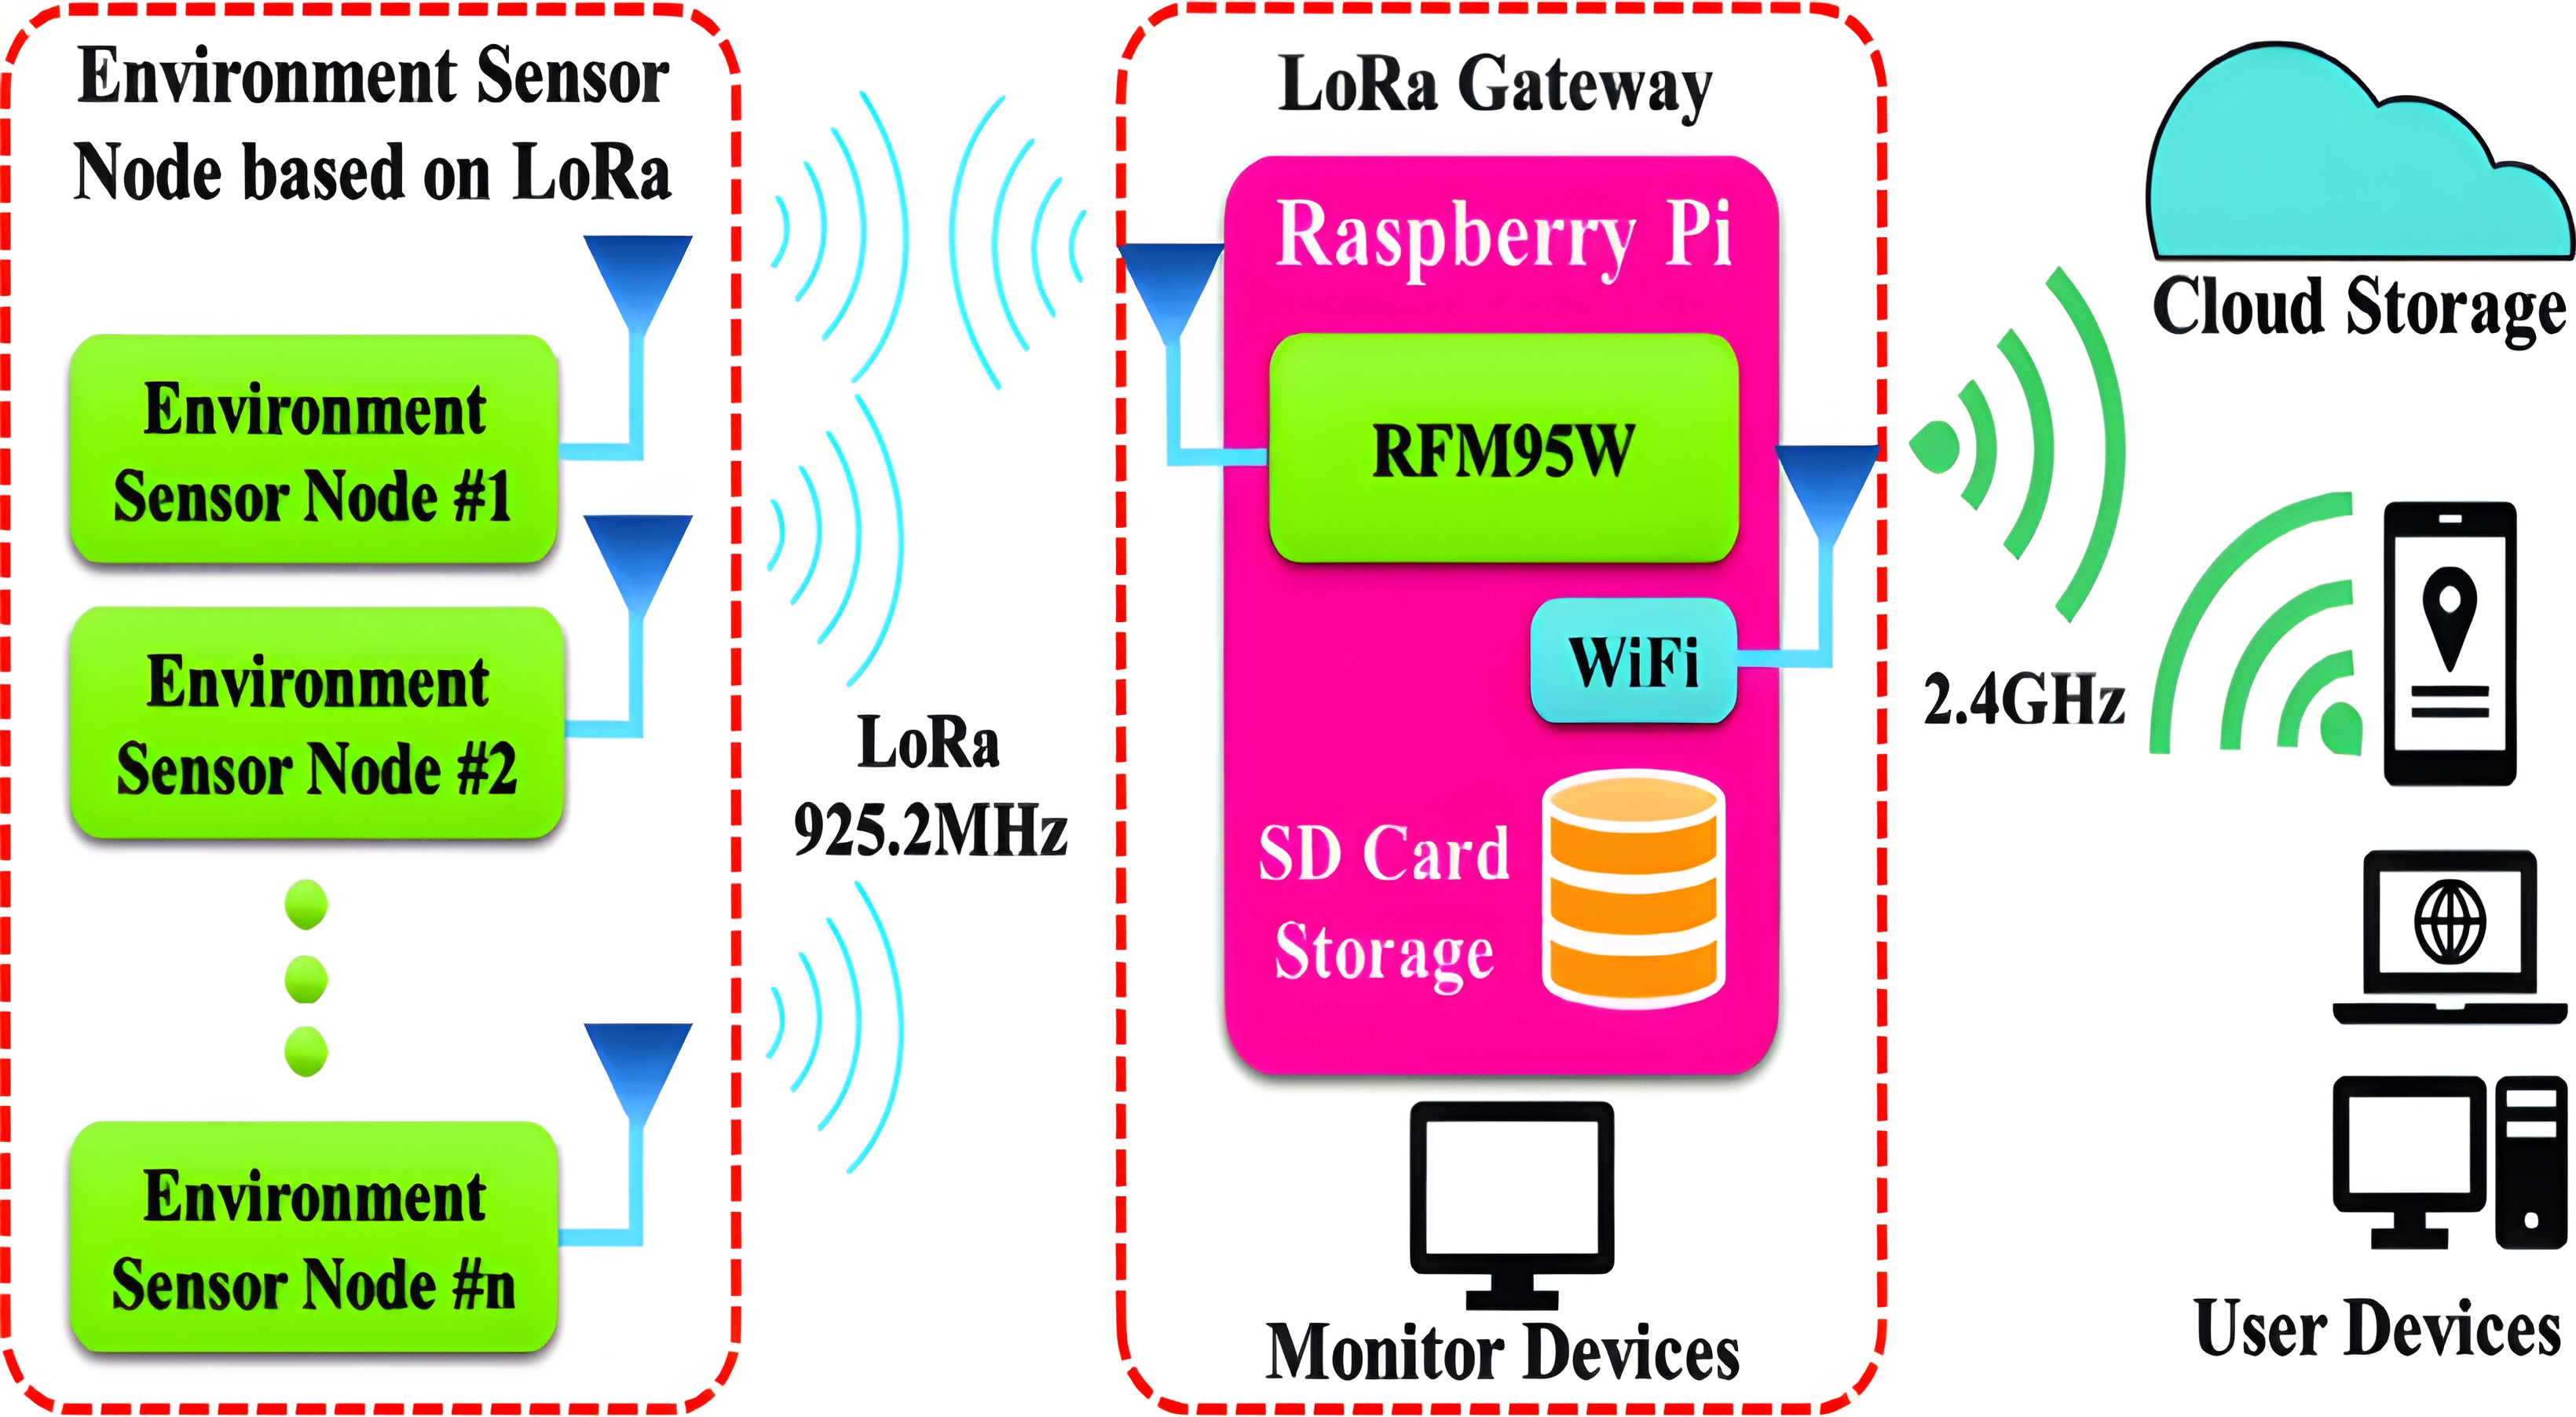
\includegraphics[scale=0.1]{Sections/Introduction/LoRaWAN-IOT-Example.jpg}
\end{figure}


\subsection{LoRa and LoRaWAN}
Low Power Wide Area Network (LPWAN) is a communication technology that offers wide coverage, similar to satellite networks, while maintaining lower data rates akin to ZigBee. The technology is distinguished by its ultra-low power consumption and cost-effective deployment and maintenance  \cite{IOTandLORAWAN-SmartFarm}.\\\\
LoRa and LoRaWAN, forms of LPWAN technology, were developed to overcome the scalabilty issues associated with traditional WSN configurations that relied on short-range communication protocols such as Zigbee and Bluetooth \cite{WSN-WaterQual}. These configurations often used a mesh network layout, which introduced challenges in network management and power consumption with increasing network size \cite{IOTandLORAWAN-SmartFarm}.\\\\
LoRaWAN's unique `star of stars' configuration addresses these challenges by enabling scalable network expansion with reduced complexity. LoRa itself is a Chirp Spread Spectrum (CSS) modulation technique developed by Cycleo, offering a Medium Access Control (MAC) protocol and operating on license-free, region-dependent Industrial, Scientific and Medical (ISM) frequency bands \cite{IOTandLORAWAN-SmartFarm}.

\begin{comment}
\begin{figure}[h]
	\centering 
	\caption{Comparison of main IoT enabling communication technologies in terms of range, data rate, energy consumption, and costs. \cite{IOTandLORAWAN-SmartFarm}}
	\label{IOTandLORAWAN-SmartFarm-Figure1}
	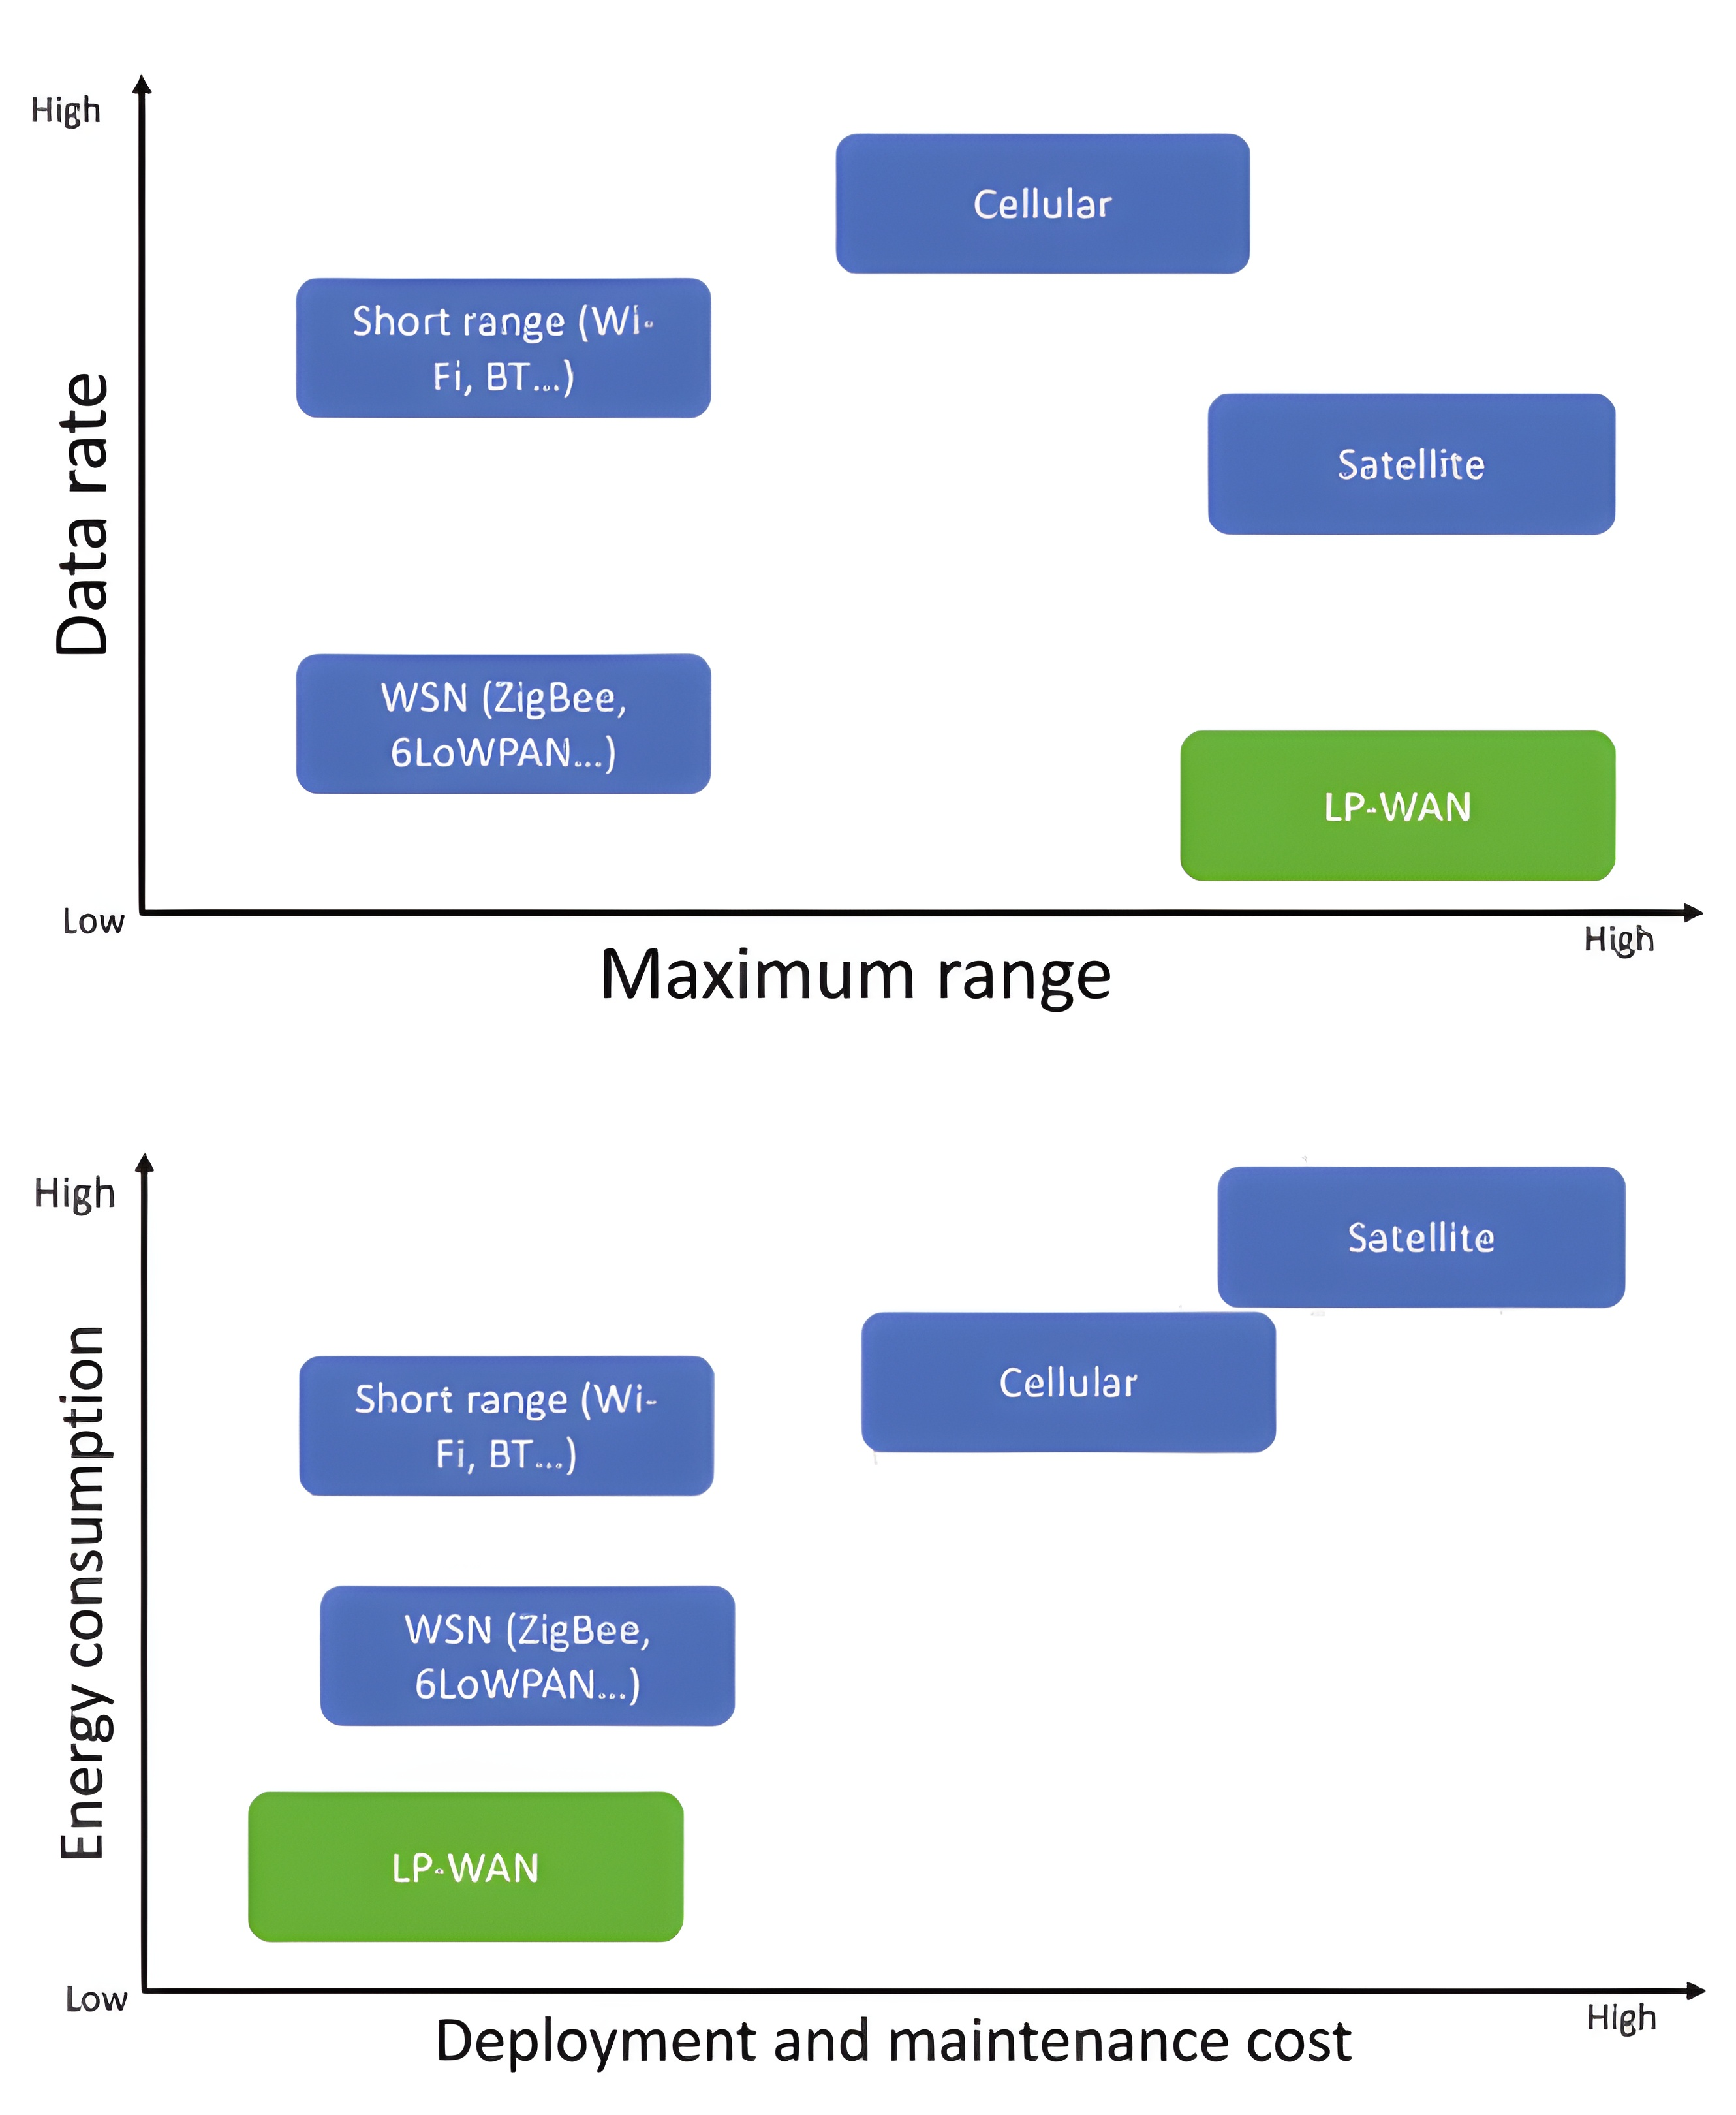
\includegraphics[scale=0.1]{Sections/Introduction/LP-WAN-Range.jpg}
\end{figure}
\end{comment}




\section{Aims and Objectives}

The aim of this project is to develop and deploy a prototype IoT architecture with the purpose of collecting data relevant to the health of the Griffith footbridge. This involves implementing the first five layers of the architecture which consist of the coding layer, perception layer, network layer, middle-ware layer and application layer. This deployment will be achieved through the testing and implementation of two prototypes.

The first prototype is designed for testing the software and the first three layers of the IoT architecture. Two Arduino MKRWAN 1300 devices will be used, one acting as the LoRa node (layer one and two) and the other acting as a pseudo LoRaWAN gateway (layer three). The first MKRWAN 1300 is equipped with an ADXL335 3-axis accelerometer and is placed on a metal beam. The beam is vibrated along the z-axis and the device samples the acceleration. The device finds the maximum frequency peak and maximum acceleration and transmits the data via a LoRa packet. The second device receives the LoRa packet and logs the data via a serial connection. The high level system diagram in figure \ref{Proto1HLSD} presents the desired implementation of this prototype. 

\begin{figure}[h]
	\centering
	\caption{Prototype 1 High Level System Diagram}
	\label{Proto1HLSD}
	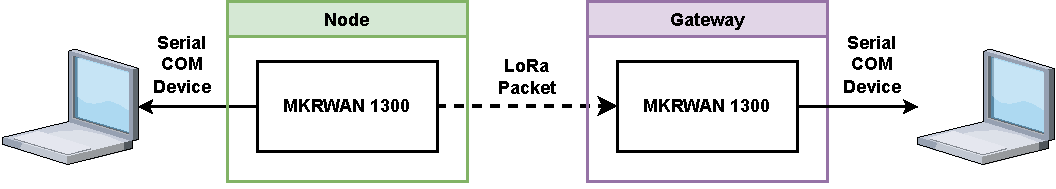
\includegraphics[scale=1]{Sections/Introduction/Prototype-1-High-Level.drawio.pdf}
\end{figure}

		The second prototype is designed for testing the software, PCB, enclosure and first five layers of the IoT architecture. The two MKRWAN 1300 devices are now both nodes and are implemented onto a custom designed PCB. This PCB is enclosed in a custom 3D printed enclosure and sits behind the guard rail of the Griffith foot bridge. The two nodes sample the maximum frequency and maximum acceleration of the bridge and transmit this data via LoRa packets to a Wisgate Edge Lite 2 LoRaWAN gateway. This gateway uploads the data via WIFI or Ethernet to the TNN cloud which acts as the middle-ware layer. --- APPLICATION LAYER WHAT IS THE IMPLEMENTATION --- Figure \ref{Proto2HLSD}
displays the high level system diagram for the second prototype. 

\begin{figure}[h] 
	\centering
	\caption{Prototype 2 High Level System Diagram}
	\label{Proto2HLSD}
	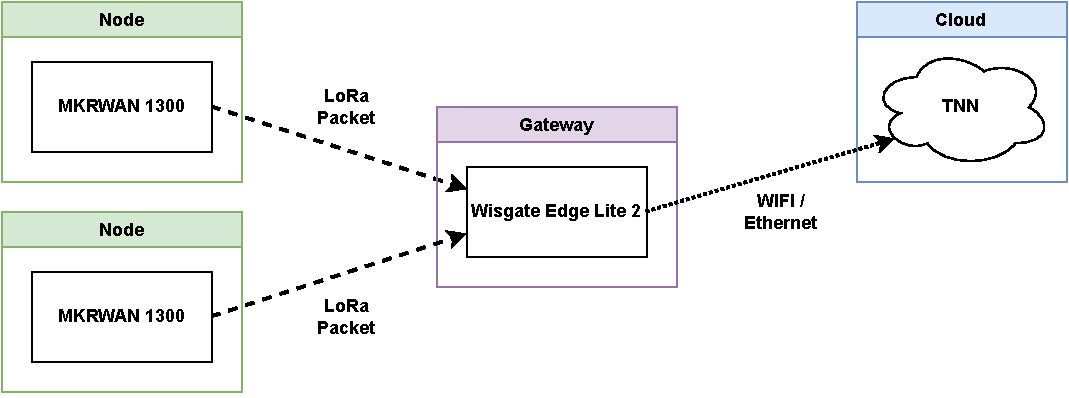
\includegraphics[scale=0.8]{Sections/Introduction/Prototype-2-High-Level.drawio.pdf}
\end{figure}

--- WHAT IS THE SUCCESS CRITERIA. SUCCESSFUL WHEN ??? ---

\newpage
\chapter{Review of Published Literature}
\section{Review of the Published Literature}
This literature review explores a variety of studies revolving around LoRaWAN and focuses on the fundamental end device setup, signal strength measurement, IoT cloud architecture and inherent limitations of the technology. LoRaWAN has gained traction for its promise of long-range, low-power solutions to WSNs which is critical for IoT applications. However, there are significant research gaps in the literature regarding the reliability and concistency of LoRaWAN in various environmental conditions and its practicality for applications requiring real time response. This review aims to evaluate these research gaps and evidence the design and optimization considerations for the LoRaWAN-based Structural Health Monitoring (SHM) deployment for the Griffith footbridge. The literature synthesized in this review is instrumental in shaping the approach and methodology of this research project. 

One application of LoRaWAN is in the field of Agro-Informatics, as demonstrated by Gehani et al. (2021) \cite{LoRa-Agro-Informatics}. Their research focused on utilizing LoRaWAN IoT architecture for the detection and classification of plant pathogens. The signal strength of the transmitted LoRa packets was evaluated through Received Signal Strength Indicator (RSSI) and Signal-to-Noise Ratio (SNR) at various depths from 0 cm to 60 cm. Their findings suggest that LoRa transmitters can function effectively provided the depth does not exceed 50 cm. A diagram of the experimental setup is shown in figure \ref{lora-bucket}. This research serves as a valuable foundation for designing the enclosure thickness that will be used in this project. 

\begin{figure}[h]
	\centering
	\caption{Experimental Setup for LoRa Node in Soil \cite{LoRa-Agro-Informatics}}
	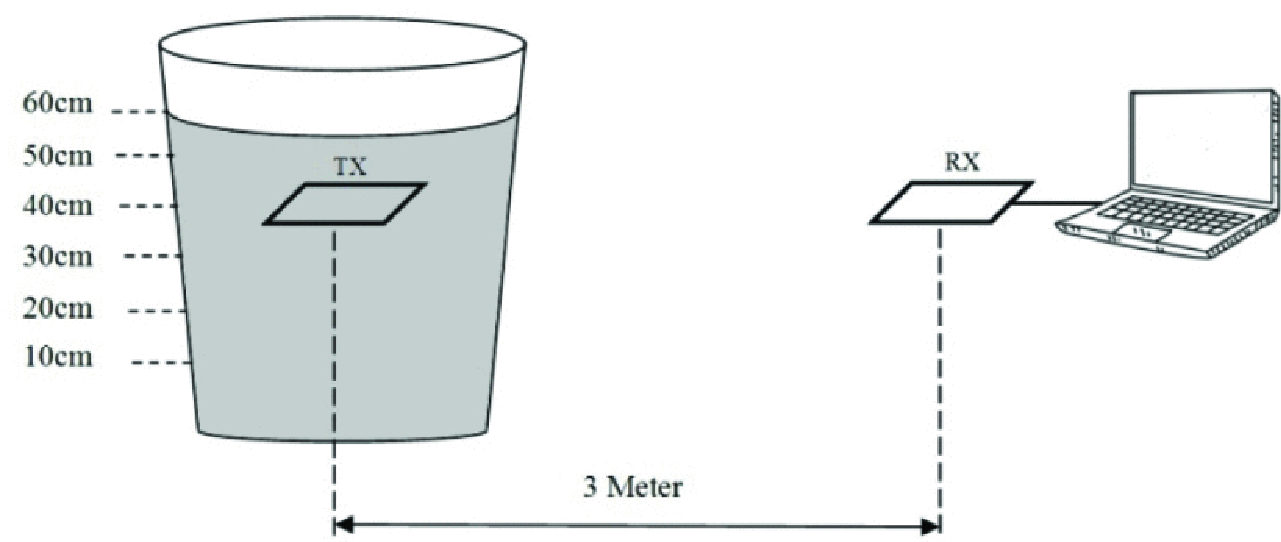
\includegraphics[scale=0.5]{Sections/Literature-Review/Lora-bucket.pdf}
	\label{lora-bucket}
\end{figure}

Fox et al. (2019) \cite{IoT-Regional-Service} expanded on the architecture of LoRaWAN-based IoT systems with a focus on wind turbine monitoring in Ireland. Their study comprised three main components: an end device, a gateway, and an IBM IoT cloud platform. This research demonstrated a comprehensive IoT cloud architecture deployment, covering real-time monitoring, concurrent read/write processes, and database service implementation. Despite the successful deployment, challenges such as LoRa's limited transmission capacity and application specific end device battery life were highlighted, emphasizing the need for future optimization. In terms of practical application, end devices must be optimized to strike a balance between computational load and current draw to achieve sufficient longevity. Figure \ref{Example-GUI} displays an example of a GUI displaying real time data visualization from the Red Node Cloud Foundry application flow within the IBM cloud. The LoRa payload is extracted, processed and displayed in an interface by assigning relative values to their respective interface nodes. With the knowledge gained from this research, the variables from the LoRa payload in this project will be extracted using Arduino IoT cloud variables, and an Arduino IoT cloud dashboard will be used to plot relevant time series data. The Arduino LoRaWAN Adaptive Data Rate (ADR) mechanism will be used in this project to optimise the airtime, data rate and power consumption of the LoRaWAN deployment. This will assist in striking the balance between computational load and current draw of the LoRa node. 

\begin{figure}[h]
	\centering
	\caption{Example of real time data visualization GUI \cite{IoT-Regional-Service}}
	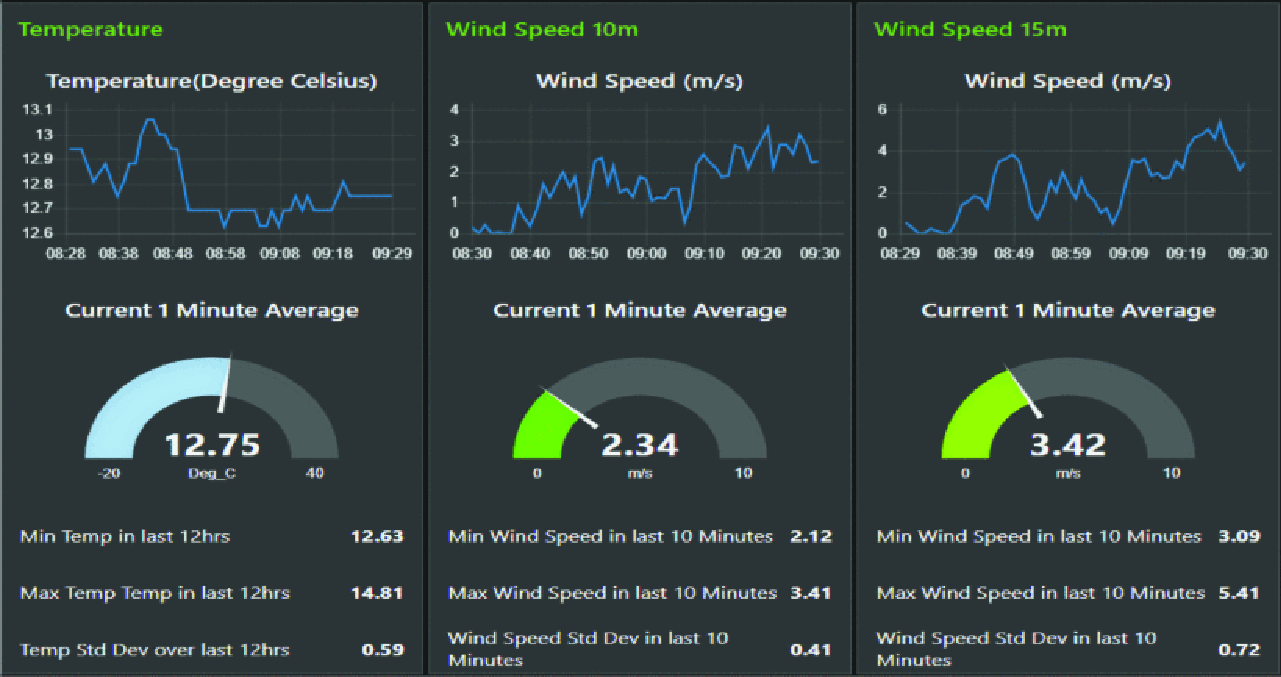
\includegraphics[scale=0.6]{Sections/Literature-Review/Example-GUI.pdf}
	\label{Example-GUI}
\end{figure}

In another exploration of LoRaWAN capabilities, Wildan et al. (2020) \cite{LoRa-Smart-Home} designed and implemented a GUI for smart home systems leveraging LoRa's long-range and low-power benefits. Information such as room temperature is transmitted to a LoRa server through a LoRa client, and is uploaded to a web server. The data is then stored in a database and displayed on a webpage which is accessible from various devices such as a smartphone and laptop. An interface application was created to allow user interaction with the webpage and control over various electronic devices such as lights, TV and air conditioning within the house. The system's performance was tested with a focus on the user experience, web application and delay. This testing was able to address a key limitation in LoRaWAN, the delay in data transmission, noting that while the system performance was generally robust, delays averaged 3.86 seconds. This makes LoRaWAN generally limited for systems that require close to real-time responses. In relation to the smart home, operating the lights and TV with a 3.86 second delay is both significant and noticeable. In its current state this system is functional, but will inevitably invoke hesitancy for mainstream adoption due to an installation cost for a user experience that is not seamless. The delay time evidenced in this study has resulted in avoiding unnecessary downlink messages for this project. This project will only focus on receiving uplink messages with only necessary downlink acknowledgements to avoid the restriction of a delayed response time. 

Maziero et al. (2019) \cite{Monitoring-Electric-Parameters} deployed a real-time monitoring system for tracking electrical quantities at the Federal University of Santa Maria campus. Utilizing Grafana software, they created a panel for tracking both electrical and connectivity metrics, demonstrating the effectiveness of combining LoRaWAN technology and application layer monitoring software for real-time data acquisition and visualization. The study highlights the potential scalability of this system in the sense of feeding data stored in the monitoring center to algorithms capable of autonomously handling the distribution network of electrical metrics, for example automatically altering voltage based on state estimations. It was evident in the research that the ability to monitor electrical quantities in the application layer allowed for the capability of better management and informed decision making based on a holistic interpretation of the distribution network. Figure \ref{Electrical-Monitoring-System} displays the design for the electrical monitoring system and the process of receiving data from The Things Network (TNN) applications and transmitting payloads to a web-based user interface via MQTT and HTTP messaging protocols. The system design of this study gives an excellent context for the chosen implementation of TNN for this project. In this project TNN applications will instead communicate with the Arduino IoT cloud using cloud variables which will be used to plot data on the web-based Arduino cloud dashboard. 

\begin{figure}[h]
	\centering
	\caption{IoT architecture for monitoring electrical quantities \cite{Monitoring-Electric-Parameters}}
	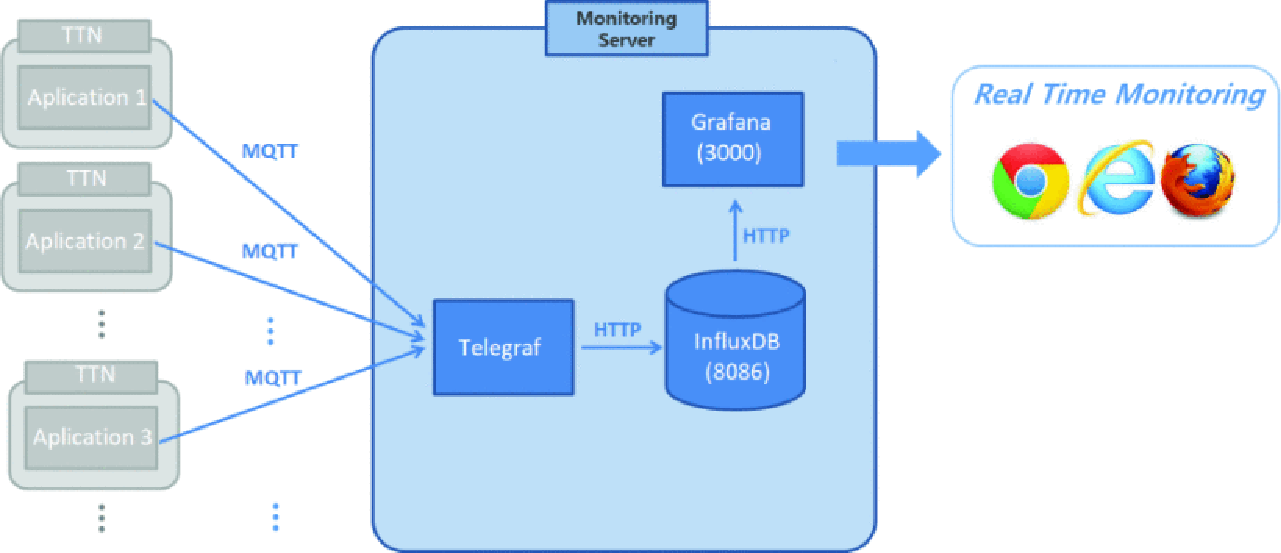
\includegraphics[scale=0.5]{Sections/Literature-Review/Electrical-Monitoring-System.pdf}
	\label{Electrical-Monitoring-System}
\end{figure}

In a study examining the performance of a Smart Gateway network architecture, the authors conducted a series of test focusing on throughput and packet loss \cite{Monitoring-System-Smart-Gateway}. The throughput was found to be inconsistent across a different number of clients where the system was found to have a lower average throughput compared to other LoRaWAN systems due to additional required processing steps. The extra processing steps were attributed to Quality of Service (QoS) parameters, such as measuring packet loss and throughput, processing client data and web server services running on the gateway. The study found a significant packet loss especially when operating with two clients. On average, the system exhibited packet loss of 26\% across a 1-meter range which is a significantly high drop compared to other LoRaWAN implementations. Despite the range limitations, the study concluded that the gateway could support up to 5 clients registering and requesting data automatically, and run LoRa communication alongside the user interface of the information system simultaneously. In light of these findings, this report intends to use the ADR mechanism to automatically optimize QoS since it dynamically chooses the best spreading factor (SF) to send LoRa packets over. Additionally, the gateway used in this project will act as a base station and use the Arduino IoT Cloud and The Things Network (TNN) to handle the network and application layer, removing unnecessary gateway computations. 

Wixted et al. (2016) \cite{LoRa-WSN} conducted reliability testing and discovered a successful connection and acknowledgement request between an end device and gateway across all spreading factors was found to be only 42\% at a distance of 1.9km. After introducing a second gateway this connection rate rose to 70\% and with the introduction of Internet Control Message protocol (ICMP) pings the full connection rate rose to 95.5\%. It was also found that connection was completely lost in isolated stairwells indicating that LoRaWAN is sensitive to obstructions. Thanks to the findings of this research, the deployment of the LoRaWAN system in this project will focus on a short-range setup with minimal obstruction, and focus on the holistic deployment of the IoT architecture. 

In a paper presenting an online test bed for LoRa development, the correlation between packet RSSI and distance was measured \cite{Dandelion-Testbed}. 5 LoRa nodes were placed at distances 500m, 1000m and 1200m away from the gateway, where the nodes placed 100m and 1200m were blocked by urban and natural obstacles. It was found that a low spreading factor (SF) results in a reduction of the packet reception rate (PRR). SF7 was the lowest spreading factor used and was confirmed to only support packet transmission at very low distance. The study concluded that RSSI decreases with distance and that this relationship is directly influenced by the environment, obstacles and spreading factor used for transmission. Various models can be used to model the relationship between RSSI and distance, but as evidenced in figure \ref{rssi-distance-model} the Bor model was closest in predicting correlation. To investigate the RSSI and SNR in this project, the values will be extracted from TNN and plotted over time series. This will further assist in gaining an understanding of the fluctuation of signal strength at a fixed distance from the Griffith footbridge. 

\begin{figure}[h]
	\centering
	\caption{Modelling RSSI-distance correlation. Green represents real data. \cite{Dandelion-Testbed}}
	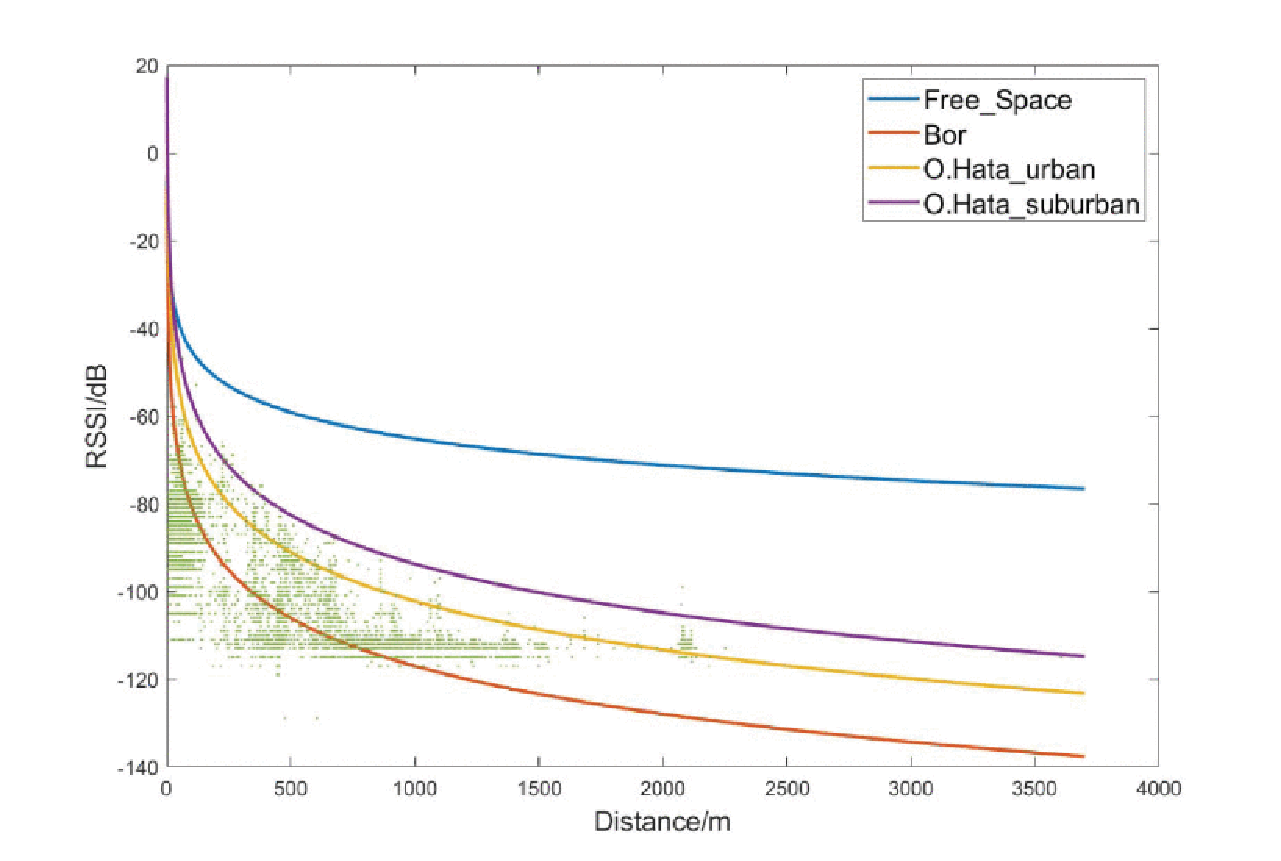
\includegraphics[scale=0.5]{Sections/Literature-Review/rssi-distance-model.pdf}
	\label{rssi-distance-model}
\end{figure}

Jang et al. in 2010 \cite{SHM-Korea} reports the deployment of 70 wireless smart sensor networks (WSSNs) and two base stations on the Jindo Bridge in South Korea. Each sensor facilitates 3-axis acceleration measurement and offers a test bed for structural health monitoring (SHM). Cho et al. in 2010 \cite{WSSN-Korean-Bridge} analysed data collected from these WSSNs, comparing these results to existing acceleration data from a wired monitoring system. The acceleration data collected from the deck and pylons of the bridge revealed a significant acceleration due to vehicle traffic. Vertical and cable vibrations were found to be significant enough for mode extraction and the estimated tension forces for 10 cables were found to lie within a 4\% difference of the previous site inspections using wired monitoring systems. The frequencies of the higher modes were found to exceed those predicted in the finite element (FE) model by less than 16\%, indicating the benefit of WSSN data collection for verifying and amending simulated models. The PSD of the 2007 site inspection using the wired monitoring system is shown in figure \ref{PSD-Wired}. This gives an excellent insight for the expected PSD frequency peaks of the Griffith footbridge, indicating that a maximum peak of approximately 2Hz may appear. 

\begin{figure}[!htb]
	\centering
	\caption{PSD of vertical acceleration with wired monitoring system \cite{WSSN-Korean-Bridge}}
	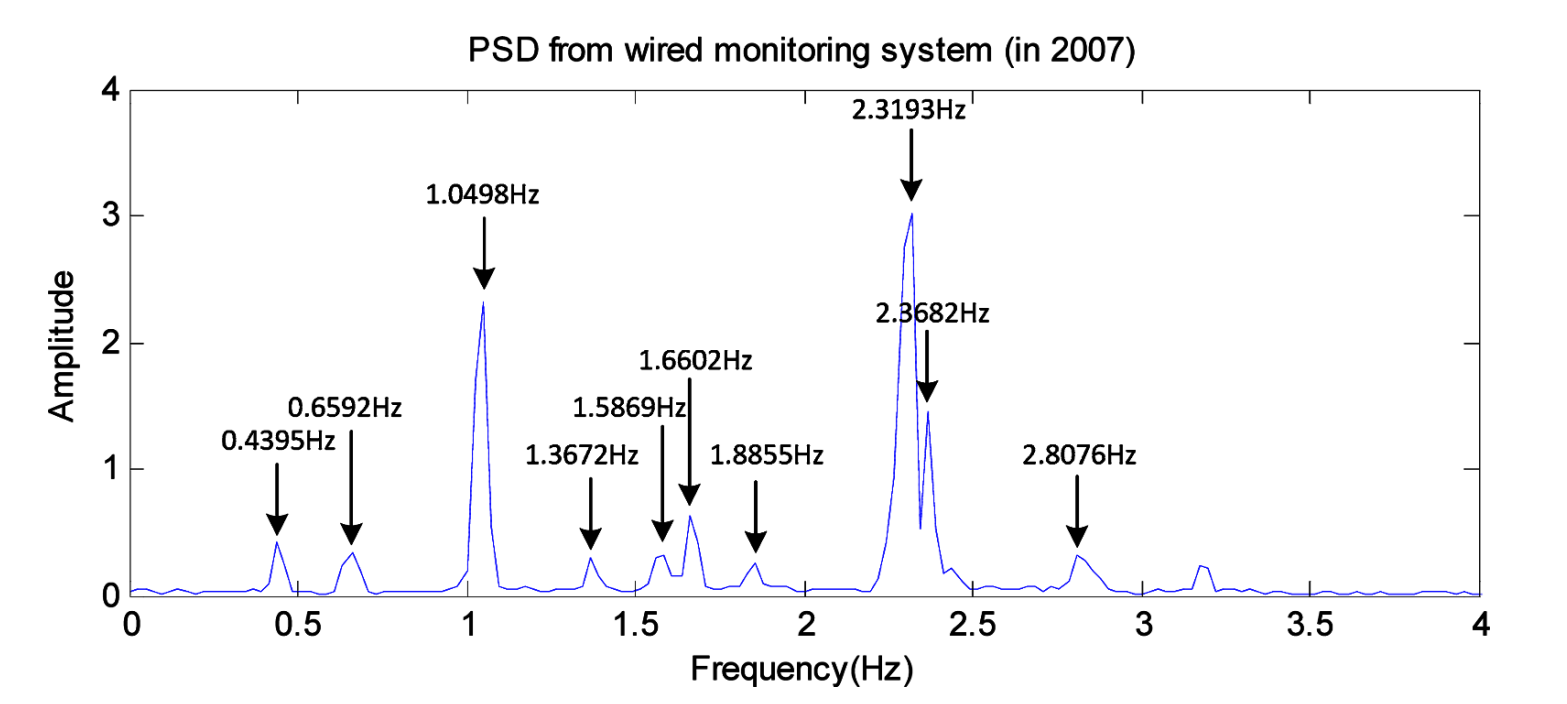
\includegraphics[scale=0.35]{Sections/Literature-Review/bridge-wired-psd.png}
	\label{PSD-Wired}
\end{figure}

The existing literature on LoRaWAN exemplifies the versatility and potential of this technology in various IoT applications, including those demanding long range and low power consumption. Several limitations including the inconsistencies in packet loss, throughput and connectivity, coupled with significant data transmission delay, as outlined in table \ref{Lit-Summary-Table}, present substantial challenges, especially for real-time data analysis and applications requiring consistent downlink messages. Such findings underscore the need for an in-depth understanding of LoRaWAN's performance to address these limitations in this project's system design. 




\begin{table}[!hbt]
\begin{tabular}{|c|l|l|}
\hline
\rowcolor[HTML]{C0C0C0} 
\textbf{Reference}                                               & \multicolumn{1}{c|}{\cellcolor[HTML]{C0C0C0}\textbf{Significant Contribution}}                                                     & \multicolumn{1}{c|}{\cellcolor[HTML]{C0C0C0}\textbf{Limitation}}                                                                                         \\ \hline
\begin{tabular}[c]{@{}c@{}}Gehani et al.\\ (2021)\end{tabular}   & \begin{tabular}[c]{@{}l@{}}LoRa Transmitters can function \\ effectively up to a depth of 50 cm\\ in soil.\end{tabular}            & \begin{tabular}[c]{@{}l@{}}Only 3 m distance between \\ transmitting and receiving \\ node.\end{tabular}                                                 \\ \hline
\begin{tabular}[c]{@{}c@{}}Fox et al.\\ (2019)\end{tabular}      & \begin{tabular}[c]{@{}l@{}}Comprehensive IoT cloud \\ architecture deployment.\end{tabular}                                        & \begin{tabular}[c]{@{}l@{}}Limited transmission\\ capacity and end device \\ battery life.\end{tabular}                                                  \\ \hline
\begin{tabular}[c]{@{}c@{}}Wildan et al. \\ (2020)\end{tabular}  & \begin{tabular}[c]{@{}l@{}}Designed and implemented a GUI \\ for smart home systems leveraging \\ LoRa.\end{tabular}               & \begin{tabular}[c]{@{}l@{}}Data transmission delay \\ averaged 3.86 seconds.\end{tabular}                                                                \\ \hline
\begin{tabular}[c]{@{}c@{}}Maziero et al.\\ (2019)\end{tabular}  & \begin{tabular}[c]{@{}l@{}}Real-time monitoring system for \\ tracking electrical quantities.\end{tabular}                         & \begin{tabular}[c]{@{}l@{}}No explanation for smart \\ meters with packet delivery \\ less than 95\%.\end{tabular}                                       \\ \hline
\begin{tabular}[c]{@{}c@{}}Eridani et al. \\ (2019)\end{tabular} & \begin{tabular}[c]{@{}l@{}}Conducted a series of tests focusing \\ on throughput and packet loss.\end{tabular}                     & \begin{tabular}[c]{@{}l@{}}Inconsistent throughput \\ and significant packet loss.\end{tabular}                                                          \\ \hline
\begin{tabular}[c]{@{}c@{}}Wixted et al. \\ (2016)\end{tabular}  & \begin{tabular}[c]{@{}l@{}}Successful connection and \\ acknowledgement request between \\ an end device and gateway.\end{tabular} & \begin{tabular}[c]{@{}l@{}}Connection was completely \\ lost in isolated stairwells \\ and low with only one gateway.\end{tabular}                       \\ \hline
\begin{tabular}[c]{@{}c@{}}Wang et al. \\ (2019)\end{tabular}    & \begin{tabular}[c]{@{}l@{}}Correlation between packet RSSI \\ and distance was measured.\end{tabular}                              & \begin{tabular}[c]{@{}l@{}}RSSI decreases with distance \\ and is directly influenced by \\ environment, obstacles and \\ spreading factor.\end{tabular} \\ \hline
\begin{tabular}[c]{@{}c@{}}Jang et al. \\ (2010)\end{tabular}    & \begin{tabular}[c]{@{}l@{}}Large scale deployment of WSSNs \\ and two base stations on the Jindo\\ Bridge.\end{tabular}            & \begin{tabular}[c]{@{}l@{}}Linear relationship between \\ number of requested data \\ points and communication time.\end{tabular}                        \\ \hline
\begin{tabular}[c]{@{}c@{}}Cho et al. \\ (2020)\end{tabular}     & \begin{tabular}[c]{@{}l@{}}Analysed data collected from the\\ WSSNs.\end{tabular}                                                  & \begin{tabular}[c]{@{}l@{}}Independent WSSN analysis \\ required due to no \\ synchronization.\end{tabular}                                              \\ \hline
\end{tabular}
\caption{Summary of Reviewed Literature}
\label{Lit-Summary-Table}
\end{table}

In the context of SHM, LoRaWAN presents a compelling alternative to traditional WSNs, such as Wi-Fi, Bluetooth and Zigbee, offering superior range and adaptability whilst satisfying low power requirements and the potential for flexible sensor placement. However, the highlighted limitations from the literature must be carefully addressed in the design of this LoRaWAN-based SHM system. This project will seek to tackle the presented challenges by focusing on the design optimization for the Griffith footbridge monitoring system. In particular, the aim is to strike a balance between computational load, power consumption and data transmission delay whilst ensuring robust and reliable system performance. 

% IMPORTANT: Latex special characters are: # $ % & \ ^ _ { } ~. To avoid mistakes when compiling try writing \ before. For: \ use \textbackslash ; for ^ \textasciitilde and ~ \textasciicircum.

%     Example of figure:
%     \begin{figure}[H]
%     	\ffigbox[\FBwidth] {
%     	\caption[Name as seen in index]{Figure name}
%     	}
%     	{\includegraphics[scale=0.6]{imagenes/creativecommons.png}}
%     \end{figure}
    

%     Example of table:
% \begin{table}[H]
% 	\ttabbox[\FBwidth]
% 	{\caption{Lorem ipsum}}
% 	{\begin{tabular}{|c|P{1.5cm}|c|P{1.5cm}|P{2cm}|c|P{1.5cm}|P{2cm}|}
% 		\hline
% 		\multicolumn{2}{|c|}{\textbf{I}} & \multicolumn{2}{c|}{\textbf{II}} & \multicolumn{3}{c|}{\textbf{III}} & \textbf{IV} \\
% 		\hline
% 		x & y & x & y & x & y & x & y \\
% 		\hline
% 		10.0 & 8.04 & 10.0 & 9.14 & 10.0 & 7.46 & 8.0 & 6.58 \\
% 		\hline
% 		8.0 & 6.95 & 8.0 & 8.14 & 8.0 & 6.77 & 8.0 & 5.76 \\
% 		\hline
% 		13.0 & 7.58 & 13.0 & 8.74 & 13.0 & 12.74 & 8.0 & 7.71 \\
% 		\hline
% 		9.0 & 8.81 & 9.0 & 8.77 & 9.0 & 7.11 & 8.0 & 8.84 \\
% 		\hline
% 		11.0 & 8.33 & 11.0 & 9.26 & 11.0 & 7.81 & 8.0 & 8.47 \\
% 		\hline
% 		14.0 & 9.96 & 14.0 & 8.10 & 14.0 & 8.84 & 8.0 & 7.04 \\
% 		\hline
% 		6.0 & 7.24 & 6.0 & 6.13 & 6.0 & 6.08 & 8.0 & 5.25 \\
% 		\hline
% 		4.0 & 4.26 & 4.0 & 3.10 & 4.0 & 5.39 & 19.0 & 12.50 \\
% 		\hline
% 		12.0 & 10.84 & 12.0 & 9.13 & 12.0 & 8.15 & 8.0 & 5.56 \\
% 		\hline
% 		7.0 & 4.82 & 7.0 & 7.26 & 7.0 & 6.42 & 8.0 & 7.91 \\
% 		\hline
% 		5.0 & 5.68 & 5.0 & 4.74 & 5.0 & 5.73 & 8.0 & 6.89 \\
% 		\hline
% 		\multicolumn{5}{l}{Source: BOE}
% 	\end{tabular}}
% \end{table}


% Start writing here----------------------------------------------------


%----------
%	Bibliography
%----------	

\clearpage
%\addcontentsline{toc}{chapter}{Bibliography}

%\printbibliography
\bibliography{References}


%----------
%	Appendix
%----------	

% If your work includes Appendix, you can uncomment the following lines
%\chapter* {Appendix x}
%\pagenumbering{gobble} % Appendix pages are not numbered



\end{document}